\chapter{Das Automatisierungswerkzeuge für \LaTeX}
\label{automate}
Wenn in \LaTeX geschrieben wird kommt es sehr bald dazu, dass man für das Literaturverzeichnis \emph{Biber} benutzen möchte, da es UTF-8 fähig ist. Dies führt dazu, dass neben pdflatex ebenfalls noch biber aufgerufen werden muss. In \href{www.overleaf.com}{Overleaf} wird dies automatisch für den Nutzer getan. Für alle die jedoch auf ihrem eigenen Rechner, also lokal mit \LaTeX schreiben, bedeutet es mehrere Aufrufe durchführen zu müssen. Hierbei gibt es nun verschiedene Wege. Unter TexStudio zum Beispiel kann in den Optionen der Aufruf automatisiert werden. Dazu muss in den Build bzw. Erzeugen Einstellungen der Ablauf angepasst werden. Öffnet dazu Optionen > TexStudio Konfigurieren > Erzeugen > Standardcompiler Button um die Reihenfolge anzupassen. 
\begin{figure}[ht]
	\centering
	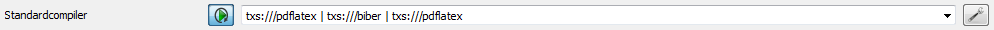
\includegraphics[width=\textwidth]{images/texstudio_option_build.PNG}
	\caption{Einstellungen für Biber in der Übersicht}
	\label{figbuild}
\end{figure}

In dem Optionsfenster \ref{figbuildOptions} kann dann die Option Biber und PdfLatex hinzugefügt werden. Für alle die kein TexStudio verwenden sondern über die Konsole ihre \LaTeX Dokumente compilieren gibt es die Automatisierungstools \emph{Arara} und \emph{LatexMK}. Diese beiden Werkzeuge werden ebenfalls häufig genutzt, wenn die Erstellung des Dokumentes sehr komplex wird und auch Dateien zwischendurch gelöscht werden müssen. Für dieses Template wurden die Optionen für \emph{Arara} bereits in die Preamble des Dokumentes hinzugefügt. Wie es benutzen ist erkläre ich im nächsten Abschnitt.

\begin{figure}[ht]
	\centering
	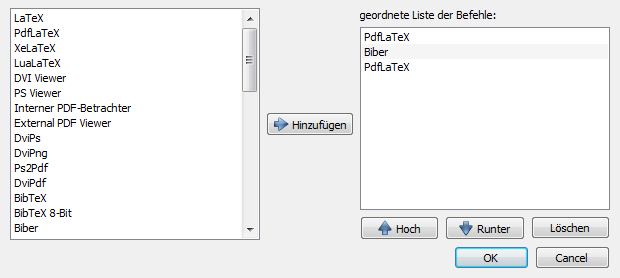
\includegraphics[width=\textwidth]{images/texstudio_optionwindow_build.PNG}
	\caption{Einstellungen für Biber im Optionsfenster}
	\label{figbuildOptions}
\end{figure}


\section{Arara}
arara ist ein TEX-Automatisierungswerkzeug, das auf Regeln und Richtlinien basiert. Es ist in mancher Hinsicht ähnlich wie andere bekannte Tools, wie z.B. latexmk\autocite{latexmk} und rubber\autocite{rubber}. Der Hauptunterschied könnte die Tatsache sein, dass arara zielt auf explizite Anweisungen im Quellcode ab, um zu ermitteln, was zu tun, anstatt sich auf andere Ressourcen, wie z.B. Logfile-Analyse, zu verlassen.
\url{https://texwelt.de/wissen/fragen/8764/was-ist-arara}
\url{https://github.com/cereda/arara}
\url{https://github.com/cereda/arara/releases}

Das Package aktivieren
Per Pakage Manager runterladen.
Dann Pfad zur Exe suchen. 
Dann das hier tun : \url{https://tex.stackexchange.com/questions/313616/configuring-arara-in-texstudio-on-windows}
Dann laufen lassen.
\url{https://latex.org/know-how/435-gnuplot-arara}
\section{LatexMK}

\url{http://mg.readthedocs.io/latexmk.html}
\url{http://personal.psu.edu/jcc8//latexmk/}
\url{http://ftp.fernuni-hagen.de/ftp-dir/pub/mirrors/www.ctan.org/support/latexmk/latexmk.pdf}

\section{Rubber}
\url{http://tex-talk.net/2011/12/building-documents-with-rubber/}
